\documentclass[12pt,a4paper]{article}
%\usepackage[table]{xcolor}
%\usepackage{float}
\usepackage[spanish]{babel}
\usepackage{lastpage}
\usepackage{enumitem}
%\usepackage{amsmath}
%\usepackage{amssymb}
\usepackage{graphicx}
%\usepackage{amsfonts}
\usepackage[utf8]{inputenx}
%\usepackage{algorithm2e}
%\usepackage{listings}
%\usepackage{pdfpages}
\usepackage{tabularx}
%\usepackage{color}
\usepackage{anysize}
\usepackage{fancyhdr}
\usepackage{ulem}
\usepackage{hyperref}
\usepackage{verbatim}
\hypersetup{
	linktoc=all
}
%\usepackage{caption}
\usepackage[font=footnotesize]{caption}
%\definecolor{deepblue}{RGB}{0,0,153}
%\definecolor{deepred}{RGB}{153,0,0}
%\definecolor{deepgreen}{RGB}{51,102,0}
%\definecolor{deepyellow}{RGB}{204,204,0}
\marginsize{2cm}{2cm}{1cm}{1.5cm} % depende de anysize
%\renewcommand*{\thefootnote}{\Roman{footnote}}
%\lstset{ %
%			language=Python,
%			basicstyle=\footnotesize,
%			numbers=left,
%			stepnumber=1,
%			numbersep=4pt,
%			tabsize=2,
%			otherkeywords={self}, 
%			keywordstyle=\color{deepred},
%			stringstyle=\color{deepgreen},
%			commentstyle=\color{deepblue},
%}
%\usepackage{hyperref}
%\hypersetup{
%    colorlinks=true,
%    citecolor=black,
%    filecolor=black,
%    linkcolor=black,
%    urlcolor=black,
%    linktoc=all
%}


\renewcommand{\footrulewidth}{0.4pt}% default is 0pt
%\title{Multímetros en Corriente Continua}
\title{
\includegraphics[scale=0.3]{images/fiuba.pdf}\\
		Universidad de Buenos Aires - FIUBA \\
		Análisis de la Información \\
		IR-TOUR\\\\
		\large{Grupo 2}}
\author{
        Gayoso, Gabriel\\
        Neira, Eduardo\\
        Pernin, Alejandro\\
        Segui, Joaquín
        \and
       	Keklikian, Nicolás\\
       	Nitz, Fernando\\
       	Salas, Cristian\\
       	}
\date{}
\pagestyle{fancy}
\lhead{1er Cuatrimestre 2015 \\ Grupo 2}
\rhead{
\includegraphics[scale=0.2]{images/FIUBA_ALTA.jpg}}
\cfoot{}
\lfoot{Gayoso - Keklikian - Neira - Nitz - Pernin - Salas - Segui}
\rfoot{\thepage/\pageref{LastPage}}
%\lfoot{asdasd}

\newenvironment{myitemize}
{\begin{itemize}[leftmargin=*,noitemsep,topsep=0pt]}{\end{itemize}}

\newenvironment{caseuse}
{\begin{center}\begin{tabular}{|l|p{10cm}|}}{\end{tabular}\end{center}}

\begin{document}
%\includepdf{attachments/caratula.pdf}


%\newpage\null\thispagestyle{empty}\newpage
\maketitle\thispagestyle{empty}

\newpage\null\thispagestyle{empty}\newpage

\newpage
\tableofcontents

\newpage\null\thispagestyle{empty}\newpage

\section{Modelo de Negocio}
	\subsection{Objetivo}
		El objetivo del sistema es organizar tours alrededor del mundo, hacer reservas, contratar excursiones, vuelos y micros. Gestionar la facturación, negociar con proveedores y mantener actualizados a los clientes de las distintas ofertas o promociones.

	\subsection{Hipótesis y Supuestos}
		\begin{itemize}
			\item Solo se realiza una anulación en caso de fuerza mayor por parte del proveedor o la no aceptación de nuevos términos por parte del cliente.
			\item Las reservas se efectúan luego de confeccionar el contrato.
			\item Los pagos son en cuotas fijas, sin inflación.
			\item En caso de cancelación, la devolución de los pagos se realizará en un pago.
			\item La modificación de un tour para un cliente no implica un cambio en la tarifa.
			\item Los clientes siempre pagan antes de la fecha de vencimiento de cada cuota.
			\item Los clientes poseen al menos un medio de pago válido.
			\item La empresa posee los contactos necesarios para satisfacer la demanda general de viáticos, hospedajes y tours.
			\item La empresa siempre puede contratar nuevos servicios o alternativas.
			\item Los clientes regulares tienen al menos un medio de contacto para recibir ofertas.
			\item El cliente retira las órdenes de servicio luego de haber abonado las cuotas correspondientes.
		\end{itemize}

	\newpage
	\subsection{Diagrama de Actividad}
		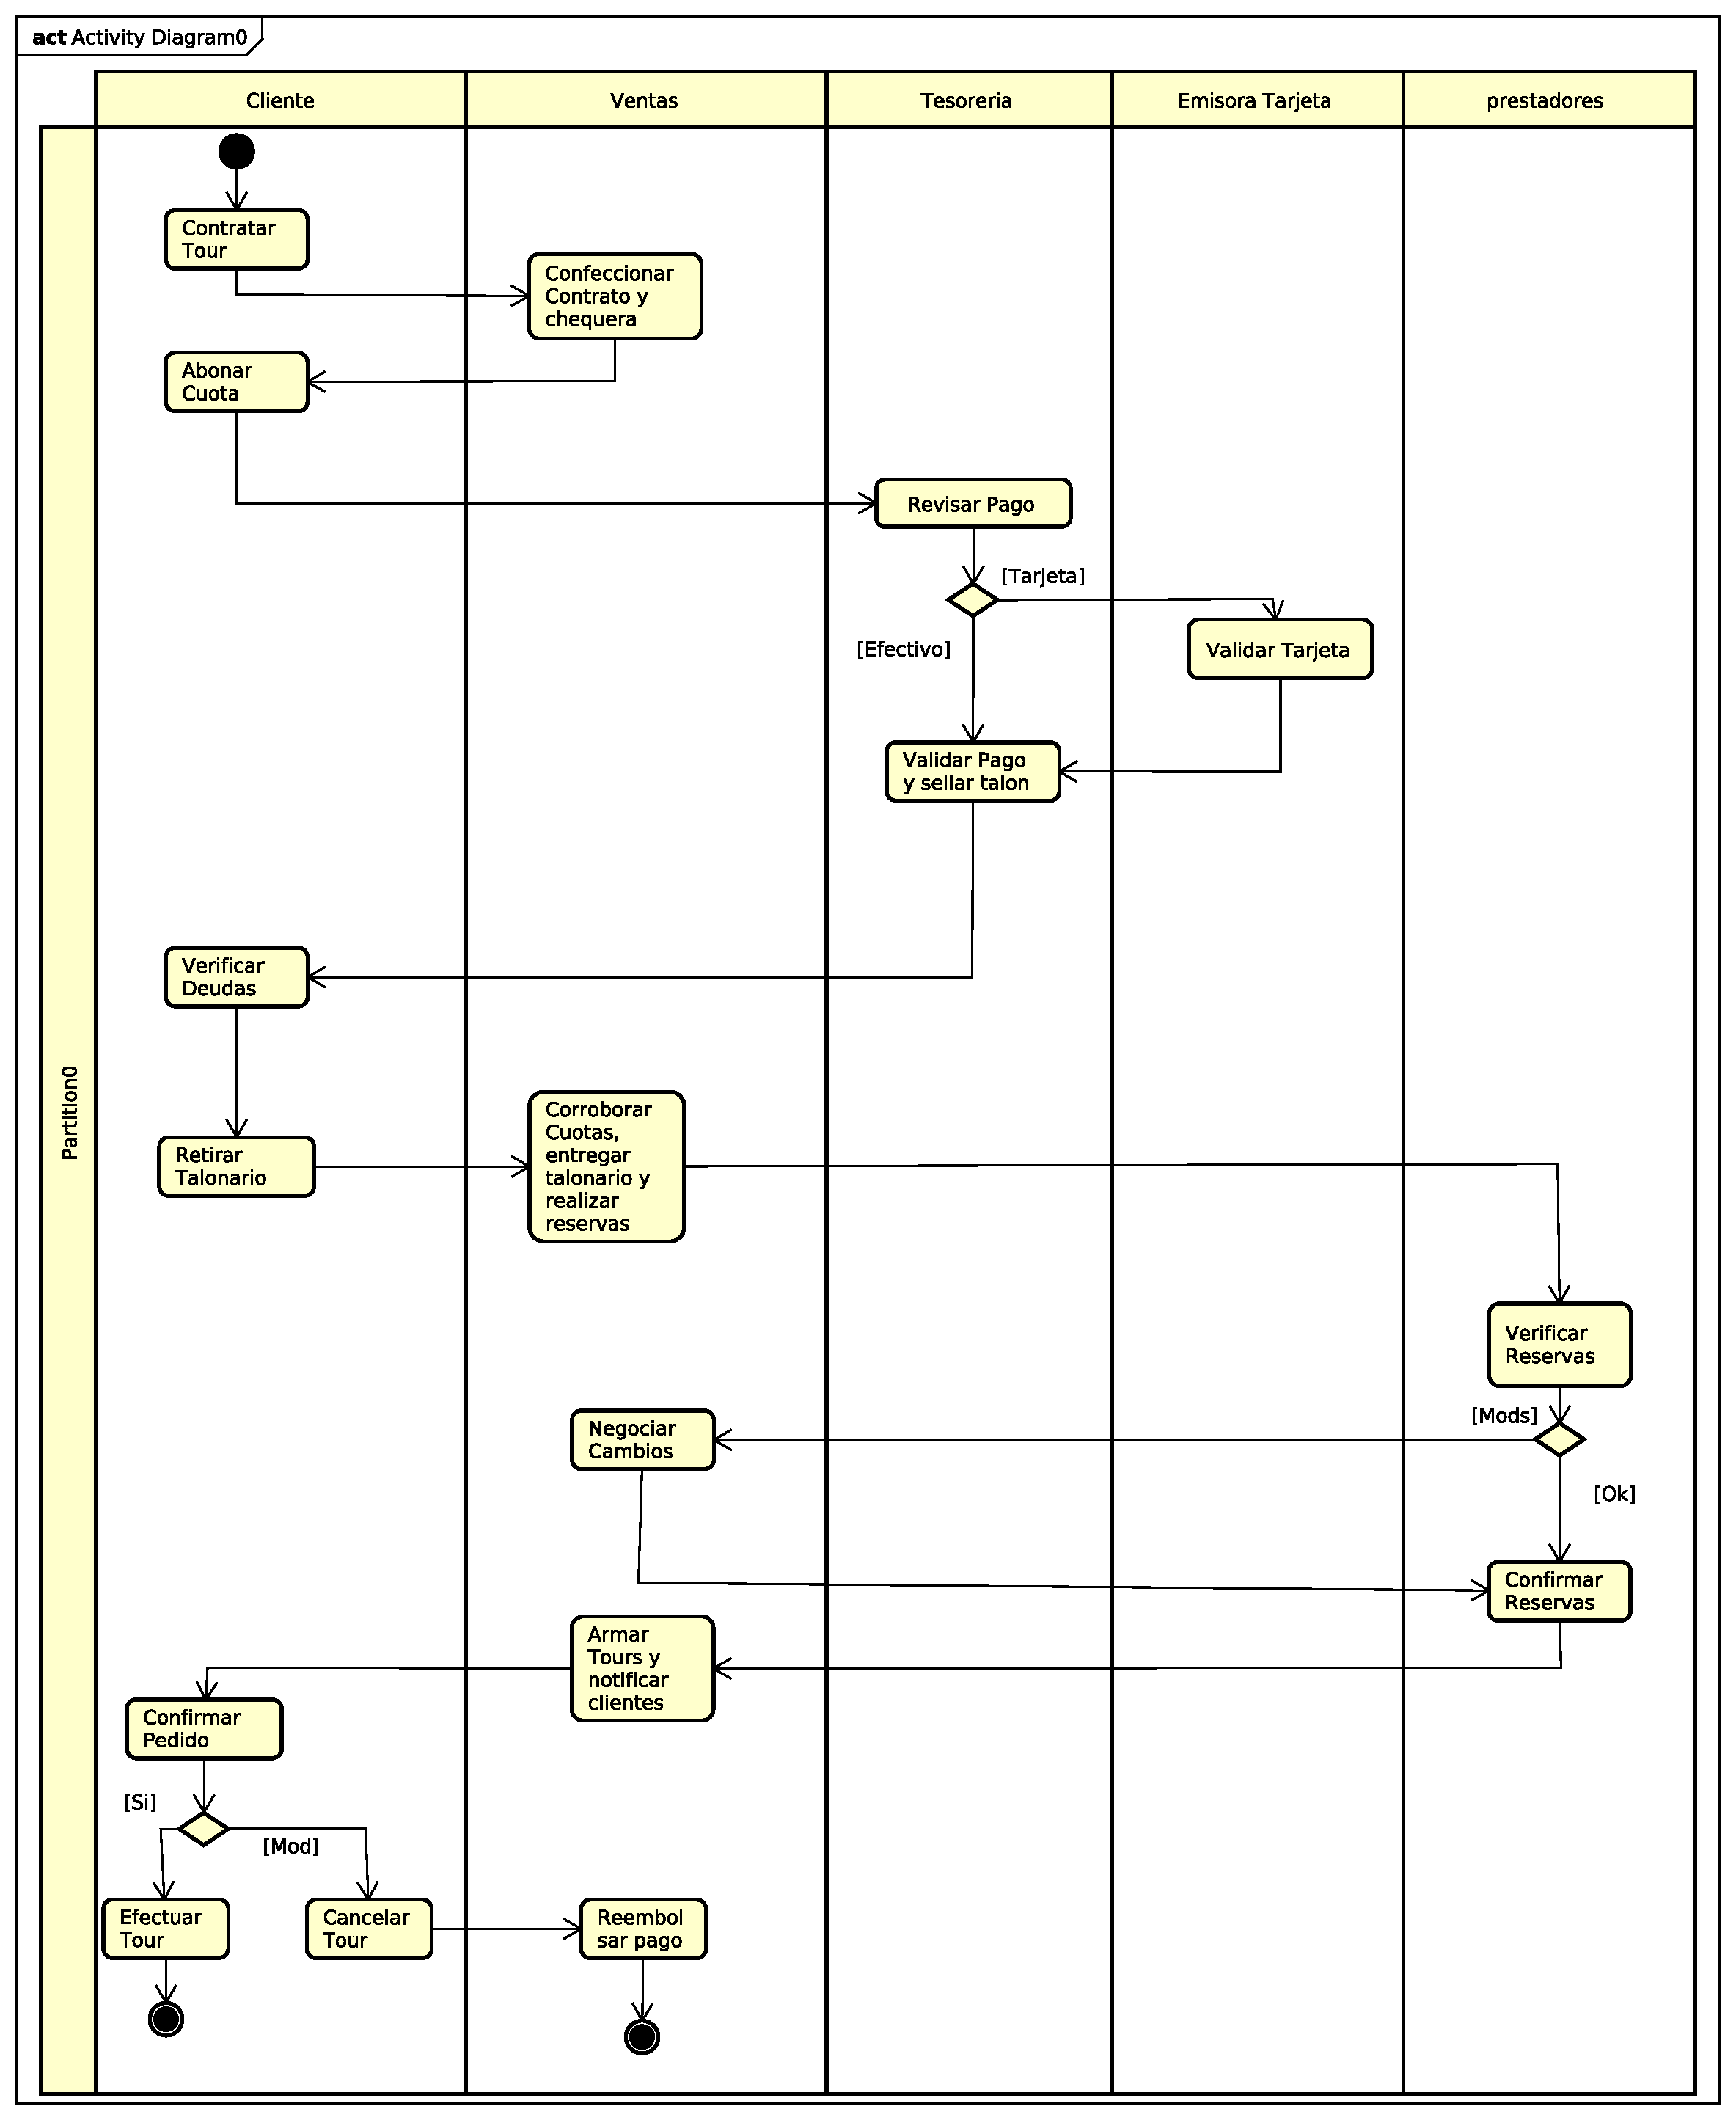
\includegraphics[scale=0.45]{images/Activity_Diagram0.pdf}

\newpage
\section{Modelo de Casos de Uso}
	\subsection{Identificación de Actores}
		\begin{itemize}
			\item \textbf{Cliente:} Es la persona que efectúa la contratación de un tour con la empresa.
			\item \textbf{Entidad Bancaria:} Es la entidad bancaria encargada de corroborar los pagos efectuados mediante tarjeta de crédito.
			\item \textbf{Administrador:} El encargado de mantener los clientes y los tours.
			\item \textbf{Prestadores:} Son quienes prestan los servicios incluidos en los tours.
			\item \textbf{Temporales:} Son aquellos que se ejecutan durante un lapso de tiempo para realizar una tarea específica.
		\end{itemize}

	\subsection{Identificación de Casos de Uso}
		\begin{itemize}
			\item \textbf{Contratar Tour:} Proceso por el cuál un cliente define el destino, las excursiones y el traslado. Se fijan las condiciones del servicio y se entrega una chequera de pago en caso de estar todo bien, caso contrario, se descarta el contrato.

			\item \textbf{Abonar Cuota:} Mensualmente, el cliente deberá abonar cada una de sus cuotas, en efectivo o con tarjeta de crédito previa validación de la entidad bancaria. 

			\item \textbf{Verificar Estado del Tour:} El cliente podrá verificar el estado del tour en todo momento. Esto implica darle información del estado del traslado, las reservas hoteleras, las excursiones y los pagos realizados.

			\item \textbf{Retirar Talonario:} Antes de realizar el tour, el cliente deberá retirar el talón con las órdenes de servicio correspondientes. Previamente se deberá corroborar que el cliente posea todas sus cuotas pagas mediante la chequera sellada.

			\item \textbf{Devolución de Pagos:} En el caso de que el cliente haya abonado el tour y los servicios no se encuentren disponibles, se le devolverá el importe completo si así lo requiere, previa validación del monto mediante la chequera.

			\item \textbf{Reservar Servicios:} Luego de que el cliente contrate un tour, se prodecerá a la reserva de los servicios correspondiantes al mismo.

			\item \textbf{Armar Tour:} Ante modificaciones por parte de los prestadores de servicios (cambios, demoras o anulaciones), se deberán armar los nuevos tours con la información nueva.

			\item \textbf{Notificar Novedades:} En caso de que los prestadores presente modificaciones que afecten los requerimientos del cliente, se les notificará permitiéndoles confirmar, modificar o anular las reservas.

			\item \textbf{Enviar Promociones y Ofertas:} Mensualmente, se deberá informar a los clientes habituales de las promociones y ofertas vigentes.

			\item \textbf{Mantener Cliente:} Se deberá tener actualizado el registro de clientes para conservar el contacto. Esto implica estar informado y mantener comunicación por algún medio de comunicación (fax, correo, e-mail u otros). 

			\item \textbf{Mantener Tour:} Se deberá tener actualizado el registro de los tours, para poder tener actualizadas las ofertas. Esto implica tener comunicación con los proveedores de servicios.

			\item \textbf{Comunicar Modificaciones:} El proveedor de un servicio comunica modificaciones de los mismos (demoras, cancelaciones o modificaciones).
		\end{itemize}

	\subsection{Descripción Casos de Uso}
		\subsubsection{Retirar Talonario}
			
		\begin{center}
			\begin{tabular}{|l|p{10cm}|}
				\hline
				\multicolumn{2}{|c|}{Retirar Talonario}\\ \hline
				Descripción & Cuando un cliente va a efectuar un tour, retira de la agencia un talonario con todas las órdenes de servicios de excurciones y pasajes correspondientes. \\ \hline

				Actores & Cliente. \\ \hline

				Pre-Condiciones & 
					\begin{itemize}[leftmargin=*,noitemsep,topsep=0pt]
						\item Antes de que el cliente efectue un tour, deberá retirar el talón con todas las órdenes de servicio para los hoteles, excursiones y pasajes correspondientes.
						\item Antes de entregar el talonario, se deberá corroborar que el cliente tenga todas sus cuotas pagas mediante la chequera sellada.
					\end{itemize}
					\\ \hline

				\multicolumn{2}{|c|}{Flujos} \\ \hline

				Flujo Principal & 
					\begin{itemize}[leftmargin=*,noitemsep,topsep=0pt]
						\item El cliente decide efectuar el tour.
						\item El cliente retira de la agencia el talonario con las ordenes de servicio.
						\item El vendedor corrobora que el cliente tenga sus cuotas abonadas. EN caso de que tenga todas sus cuotas abonadas, se procede con el subflujo A, en caso contrario con el subflujo B.
						\item Fin.
					\end{itemize}\\ \hline

				\multicolumn{2}{|c|}{Flujos Alternativos} \\ \hline

				Subflujo A & 
					\begin{itemize}[leftmargin=*,noitemsep,topsep=0pt]
						\item Se concreta la operación
						\item Fin
					\end{itemize} \\ \hline

				Subflujo B &
					\begin{myitemize}
						\item Si el cliente no tiene abonadas todas las cuotas, no se podrá retirar el talonario.
						\item Fin
					\end{myitemize} \\ \hline

				Post-Condiciones & 
					\begin{myitemize}
						\item El cliente posee 
					\end{myitemize}\\ \hline
			\end{tabular}
		\end{center}

		\subsubsection{Abonar Cuota}

			\begin{caseuse}
				\hline
				\multicolumn{2}{|c|}{Abonar Cuota} \\ \hline

				Descripción & Mensualmente, el cliente deberá pagar cada una de sus cuotas, en efectivo o tarjeta de crédito. \\ \hline

				Actores & Cliente, Entida Bancaria. \\ \hline

				Pre-Condiciones &
					\begin{myitemize}
						\item El empleado de la agencia deberá chequear el importe a pagar en dicha fecha.
					\end{myitemize}\\ \hline

				\multicolumn{2}{|c|}{Flujos} \\ \hline

				Flujo Principal &
					\begin{myitemize}
						\item En la fecha principal de cada cuota, el cliente la abona en tesorería.
						\item Fin.
					\end{myitemize} \\ \hline

				\multicolumn{2}{|c|}{Flujos Alternativos} \\ \hline

				Subflujo A & 
					\begin{myitemize}
						\item En caso de pagar en efectivo, se deberá sellar el talonario correspondiente a la fecha. Se continua el flujo en Fin de flujo principal.
						\item Fin.
					\end{myitemize} \\ \hline

				Subflujo B &
					\begin{myitemize}
						\item En caso de pagar con tarjeta de crédito, se deberá chequear la misma con la entidad bancaria y confeccionar el cupón de pago correspondiente y entregar el original.
						\item Fin.
					\end{myitemize} \\ \hline

				Post-Condiciones & El cliente posee una cuota del viaje paga.\\ \hline
			\end{caseuse}

		\subsubsection{Verificar Estado del Tour}

			\begin{caseuse}
				\hline
				\multicolumn{2}{|c|}{Verificar Estado del Tour} \\ \hline

				Descripción & El cliente podrá chequear el estado del tour en todo momento. Esto implica, darle información del estado del traslado, las reservas hoteleras, las excursiones y de los pagos hechos hasta el momento. \\ \hline

				Actores & Cliente. \\ \hline

				Pre-Condiciones & 
					\begin{myitemize}
						\item Anteriormente se debe haber seservado un tour.
					\end{myitemize} \\ \hline

				\multicolumn{2}{|c|}{Flujos} \\ \hline

				Flujo Principal &
					\begin{myitemize}
						\item El cliente verifica el estado actual del tour, lo cual implica el estado de los servicios, pasajes y reservas hoteleras.
						\item Fin.
					\end{myitemize} \\ \hline

				\multicolumn{2}{|c|}{Flujos Alternativos} \\ \hline

				Subflujo A & 
					\begin{myitemize}
						\item De haber alguna modificación el cliente puede optar por aceptarla o pedir un reembolso. De solicitarlo se continúa en Devolver Pago.
						\item Fin.
					\end{myitemize} \\ \hline

				Post-Condiciones &
					\begin{myitemize}
						\item El cliente posee el estado actualizado del tour.
					\end{myitemize}\\ \hline
			\end{caseuse}


		\subsubsection{Devolver Pago}

			\begin{caseuse}
				\hline
				\multicolumn{2}{|c|}{Devolver Pago} \\ \hline

				Descripción & En caso de que el cliente haya abonado el tour y no se le pueda brindar el servicio que requiere, se le devolverá el pago en su totalidad. \\ \hline

				Actores & Cliente, Entidad Bancaria. \\ \hline

				Pre-Condiciones & 
					\begin{myitemize}
						\item Se deberá validad el monto que figura en la chequera y los pagos realizados.
					\end{myitemize} \\ \hline

				\multicolumn{2}{|c|}{Flujos} \\ \hline

				Flujo Principal &
					\begin{myitemize}
						\item El cliente reclama por un servicio insatisfecho.
						\item Se presenta en la agencia para la devolución del pago.
						\item El vendedor corrobora las cuotas abonadas y el estado del servicio, y se realiza la devolución del pago.
						\item Fin.
					\end{myitemize} \\ \hline

				Post-Condiciones &
					\begin{myitemize}
						\item El cliente recupera el dinero abonado en las cuotas.
					\end{myitemize}\\ \hline
			\end{caseuse}	

		\subsubsection{Notificar Novedades}

			\begin{caseuse}
				\hline
				\multicolumn{2}{|c|}{Notificar Novedades} \\ \hline

				Descripción & Se le notificará a los clientes alcanzados por las modificaciones sobre los servicios afectados. \\ \hline

				Actores & Cliente. \\ \hline

				Pre-Condiciones & 
					\begin{myitemize}
						\item Los prestadores presentan alguna modificación (cambio, demora o anulación) en la que se vean afectadas los requerimientos de los clientes.
					\end{myitemize} \\ \hline

				\multicolumn{2}{|c|}{Flujos} \\ \hline

				Flujo Principal &
					\begin{myitemize}
						\item Se le informa al cliente de la modificación.
						\item Se le ofrecen alternativas para suplir su demanda, si acepta se procede con el subflujo A, de lo contrario con el B.
						\item Fin.
					\end{myitemize} \\ \hline

				\multicolumn{2}{|c|}{Flujos Alternativos} \\ \hline

				Subflujo A & 
					\begin{myitemize}
						\item Se realizan los cambios en el tour.
						\item Fin.
					\end{myitemize} \\ \hline

				Subflujo B & 
					\begin{myitemize}
						\item Se gestiona la devolución del dinero.
						\item Fin.
					\end{myitemize} \\ \hline

				Post-Condiciones &
					\begin{myitemize}
						\item El cliente se encuentra informado de las novedades del tour.
					\end{myitemize}\\ \hline
			\end{caseuse}


		\subsubsection{Enviar Promociones y Ofertas}

			\begin{caseuse}
				\hline
				\multicolumn{2}{|c|}{Enviar Promociones y Ofertas} \\ \hline

				Descripción & Se le notificará a los clientes de las promociones y ofertas vigentes. \\ \hline

				Actores & Cliente, Temporal: mensualmente. \\ \hline

				Pre-Condiciones & 
					\begin{myitemize}
						\item Se tiene un medio de comunicación con los clientes.
					\end{myitemize} \\ \hline

				\multicolumn{2}{|c|}{Flujos} \\ \hline

				Flujo Principal &
					\begin{myitemize}
						\item Se le informa al cliente de las ofertas y promociones a través de un medio de comunicación (mail, teléfono, etc).
						\item Fin.
					\end{myitemize} \\ \hline

				Post-Condiciones &
					\begin{myitemize}
						\item El cliente recibió la información de las ofertas.
					\end{myitemize}\\ \hline
			\end{caseuse}

		\subsubsection{Comunicar Modificaciones}

			\begin{caseuse}
				\hline
				\multicolumn{2}{|c|}{Comunicar Modificaciones} \\ \hline

				Descripción & Los prestadores de servicios presentan cambios de los servicios, disponibilidad y/o demoras. \\ \hline

				Actores & Prestadores. \\ \hline

				Pre-Condiciones & 
					\begin{myitemize}
						\item Se reservaron servicios prestados por el prestador.
					\end{myitemize} \\ \hline

				\multicolumn{2}{|c|}{Flujos} \\ \hline

				Flujo Principal &
					\begin{myitemize}
						\item Se reciben las novedades en los servicios que prestan los prestadores.
						\item Se actualizan dichos servicios.
						\item Fin.
					\end{myitemize} \\ \hline

				Post-Condiciones &
					\begin{myitemize}
						\item El sistema posee información actualizada sobre los servicios.
					\end{myitemize}\\ \hline
			\end{caseuse}


		\subsubsection{Mantener Cliente}

			\begin{caseuse}
				\hline
				\multicolumn{2}{|c|}{Mantener Cliente} \\ \hline

				Descripción & Se deberá tener actualizado el registro de los clientes para poder conservar el contacto. Esto implica estar informado y mantener comuncación por un medio de contacto. \\ \hline

				Actores & Administrador. \\ \hline

				Pre-Condiciones & 
					\begin{myitemize}
						\item Se tiene contacto con el cliente y brinda acceso a su estado.
					\end{myitemize} \\ \hline

				\multicolumn{2}{|c|}{Flujos} \\ \hline

				Flujo Principal &
					\begin{myitemize}
						\item El administrador chequea la base de datos de los clientes.
						\item Se realizan las altas, bajas y modificaciones de los respectivos clientes.
						\item Fin.
					\end{myitemize} \\ \hline

				Post-Condiciones &
					\begin{myitemize}
						\item Se tendrá actualizada la base de datos de los clientes.
					\end{myitemize}\\ \hline
			\end{caseuse}

	\subsubsection{Mantener Tour}

			\begin{caseuse}
				\hline
				\multicolumn{2}{|c|}{Mantener Tour} \\ \hline

				Descripción &  Se deberá tener actualizado el registro de los tours, para poder tener actualizadas las ofertas.\\ \hline

				Actores &  Administrador\\ \hline

				Pre-Condiciones & 
					\begin{myitemize}
						\item Se tiene contacto con el prestador y brinda acceso a su estado.
					\end{myitemize} \\ \hline

				\multicolumn{2}{|c|}{Flujos} \\ \hline

				Flujo Principal &
					\begin{myitemize}
						\item El administrador chequea la base de datos de los tours de los prestadores.
						\item Se actualizan, eliminan e incorporan tours acorde a la actualización de los servicios.
						\item Fin.
					\end{myitemize} \\ \hline

				Post-Condiciones &
					\begin{myitemize}
						\item Se tendrá actualizada la base de tours.
					\end{myitemize}\\ \hline
			\end{caseuse}	


		\subsubsection{Armar Tour}

			\begin{caseuse}
				\hline
				\multicolumn{2}{|c|}{Armar Tour} \\ \hline

				Descripción &  Se incorpora al sistema información nueva de un paquete de servicios\\ \hline

				Actores & Administrador. \\ \hline

				Pre-Condiciones & 
					\begin{myitemize}
						\item Se cuenta con la información de un tour aún no existente.
					\end{myitemize} \\ \hline

				\multicolumn{2}{|c|}{Flujos} \\ \hline

				Flujo Principal &
					\begin{myitemize}
						\item Se idea un paquete de servicios.
						\item Se carga el tour para posterior promoción.
						\item Fin.
					\end{myitemize} \\ \hline

				Post-Condiciones &
					\begin{myitemize}
						\item Se incorpora un tour al sistema.
					\end{myitemize}\\ \hline
			\end{caseuse}

	\subsubsection{Reservar Servicios}

			\begin{caseuse}
				\hline
				\multicolumn{2}{|c|}{Reservar Servicios} \\ \hline

				Descripción & Se toma contacto con los proveedores y se reservan los servicios requeridos por los clientes. \\ \hline

				Actores & Prestadores. \\ \hline

				Pre-Condiciones & 
					\begin{myitemize}
						\item El cliente realizó una reserva de un servicio.
					\end{myitemize} \\ \hline

				\multicolumn{2}{|c|}{Flujos} \\ \hline

				Flujo Principal &
					\begin{myitemize}
						\item Se contacta a los prestadores.
						\item El prestador valida que el servicio esté disponible. De estarlo se procede con el subflujo A, en caso contrario se procede con el B.
					\end{myitemize} \\ \hline

				\multicolumn{2}{|c|}{Flujos Alternativos} \\ \hline

				Subflujo A & 
					\begin{myitemize}
						\item Se reservan los servicios.
						\item Fin.
					\end{myitemize} \\ \hline

				Subflujo B & 
					\begin{myitemize}
						\item Se utilizan los servicios de otro proveedor.
						\item Fin.
					\end{myitemize} \\ \hline

				Post-Condiciones &
					\begin{myitemize}
						\item El cliente posee el tour actualizado acorde a los servicios disponibles.
					\end{myitemize}\\ \hline
			\end{caseuse}


		\subsubsection{Contratar un Tour}

			\begin{caseuse}
				\hline
				\multicolumn{2}{|c|}{Contratar un Tour} \\ \hline

				Descripción &  El cliente realiza la contratación de un tour.\\ \hline

				Actores &  Cliente.\\ \hline

				\multicolumn{2}{|c|}{Flujos} \\ \hline

				Flujo Principal &
					\begin{myitemize}
						\item El cliente realiza la contratación de un tour ofrecido por la agencia.
						\item Se establecen los términos y condiciones del mismo.
						\item Se le entrega la chequera de pagos.
						\item Fin.
					\end{myitemize} \\ \hline

				Post-Condiciones &
					\begin{myitemize}
						\item El cliente posee contratado un tour.
						\item El cliente posee su chequera de pagos.
					\end{myitemize}\\ \hline
			\end{caseuse}


\begin{comment}
\subsubsection{Notificar Novedades}

			\begin{caseuse}
				\hline
				\multicolumn{2}{|c|}{Notificar Novedades} \\ \hline

				Descripción &  \\ \hline

				Actores &  \\ \hline

				Pre-Condiciones & 
					\begin{myitemize}
					\end{myitemize} \\ \hline

				\multicolumn{2}{|c|}{Flujos} \\ \hline

				Flujo Principal &
					\begin{myitemize}
					\end{myitemize} \\ \hline

				\multicolumn{2}{|c|}{Flujos Alternativos} \\ \hline

				Subflujo A & 
					\begin{myitemize}
					\end{myitemize} \\ \hline

				Post-Condiciones &
					\begin{myitemize}
					\end{myitemize}\\ \hline
			\end{caseuse}
\end{comment}



\subsection{Diagrama de Casos de Uso}
	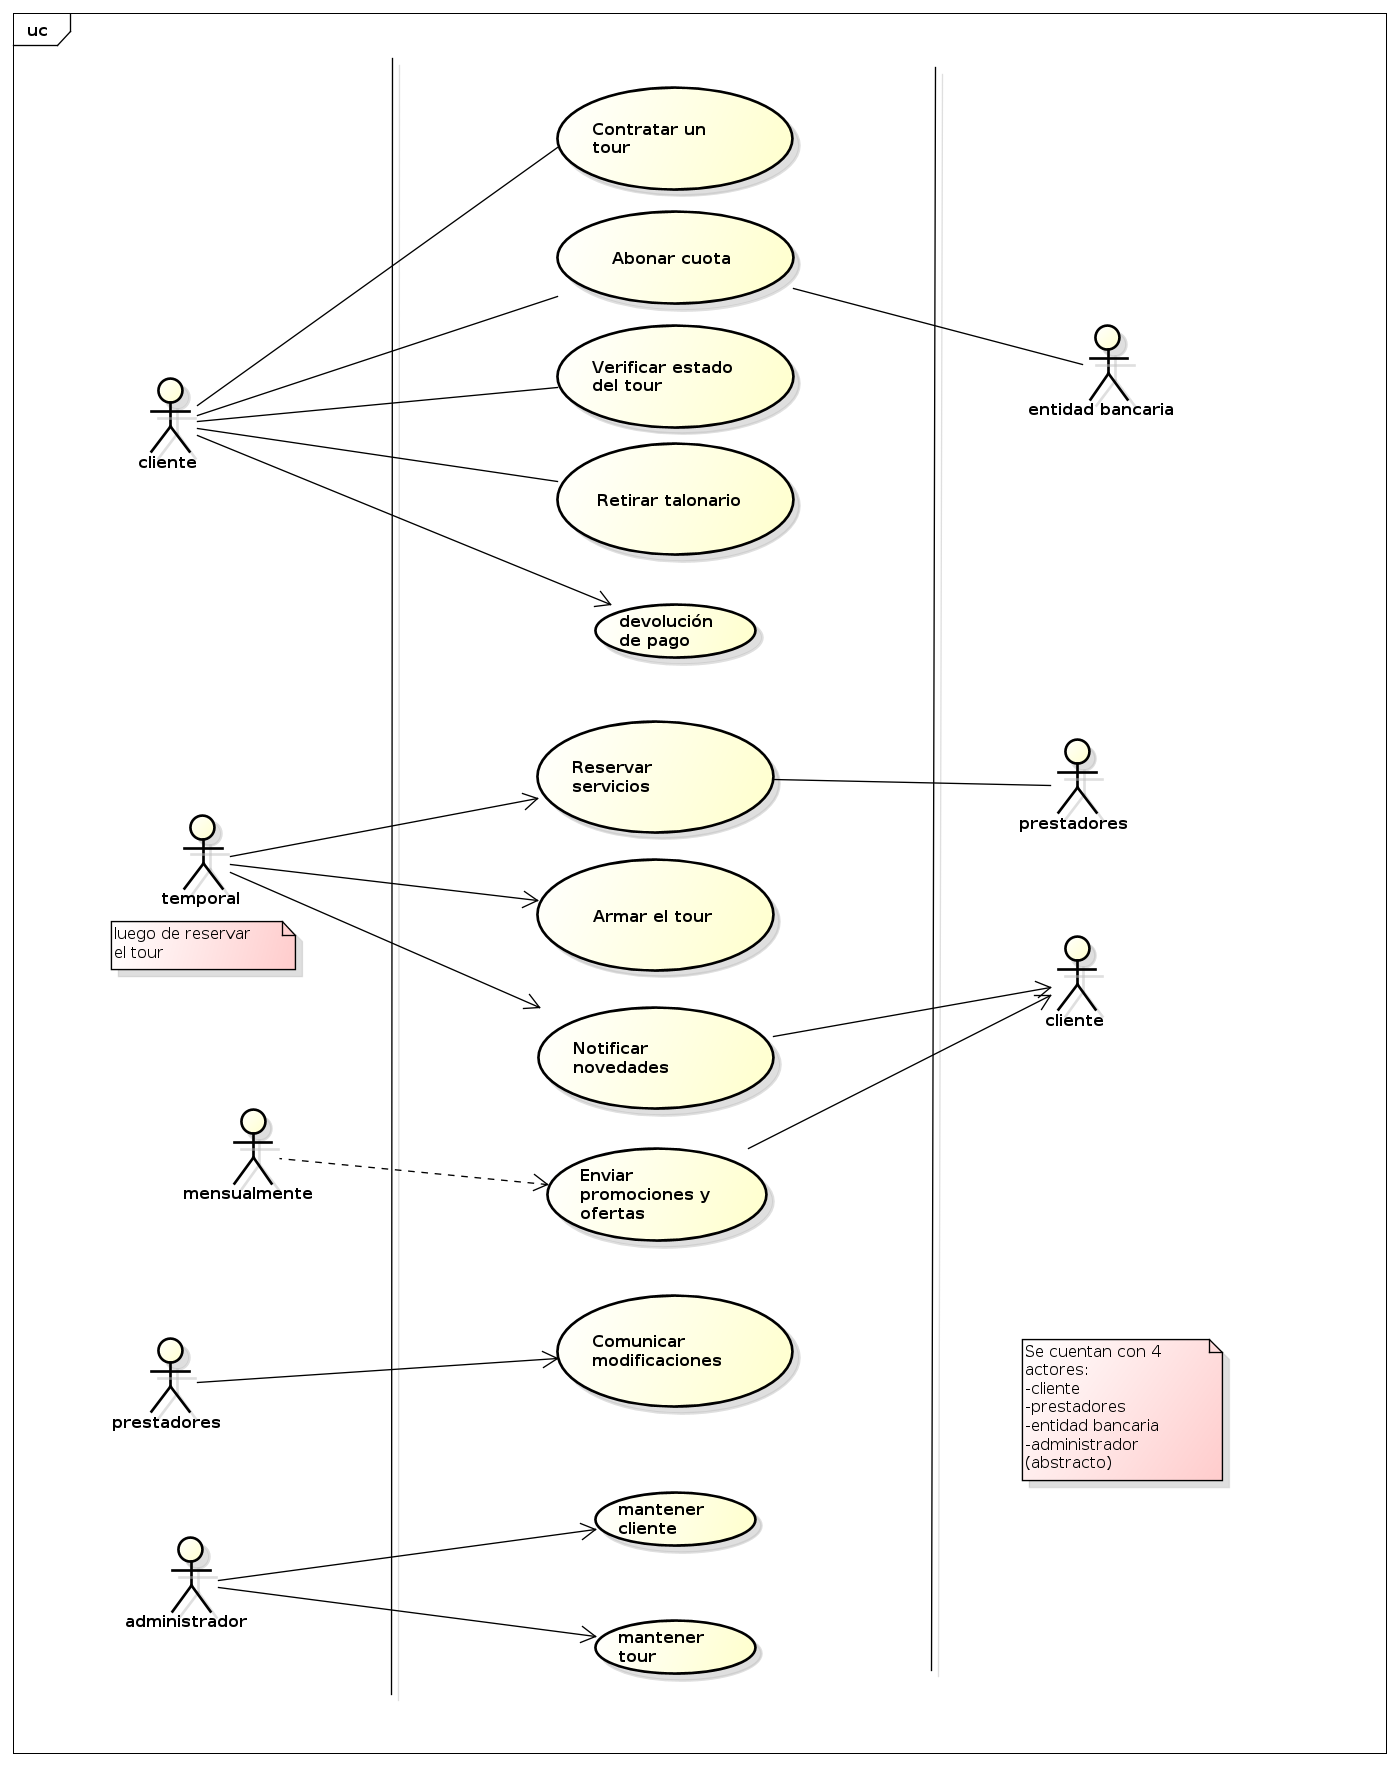
\includegraphics[scale=0.5]{images/UseCaseDiagram0.png}

\section{Modelo de Clases}
	\subsection{Diagrama de Clases}
		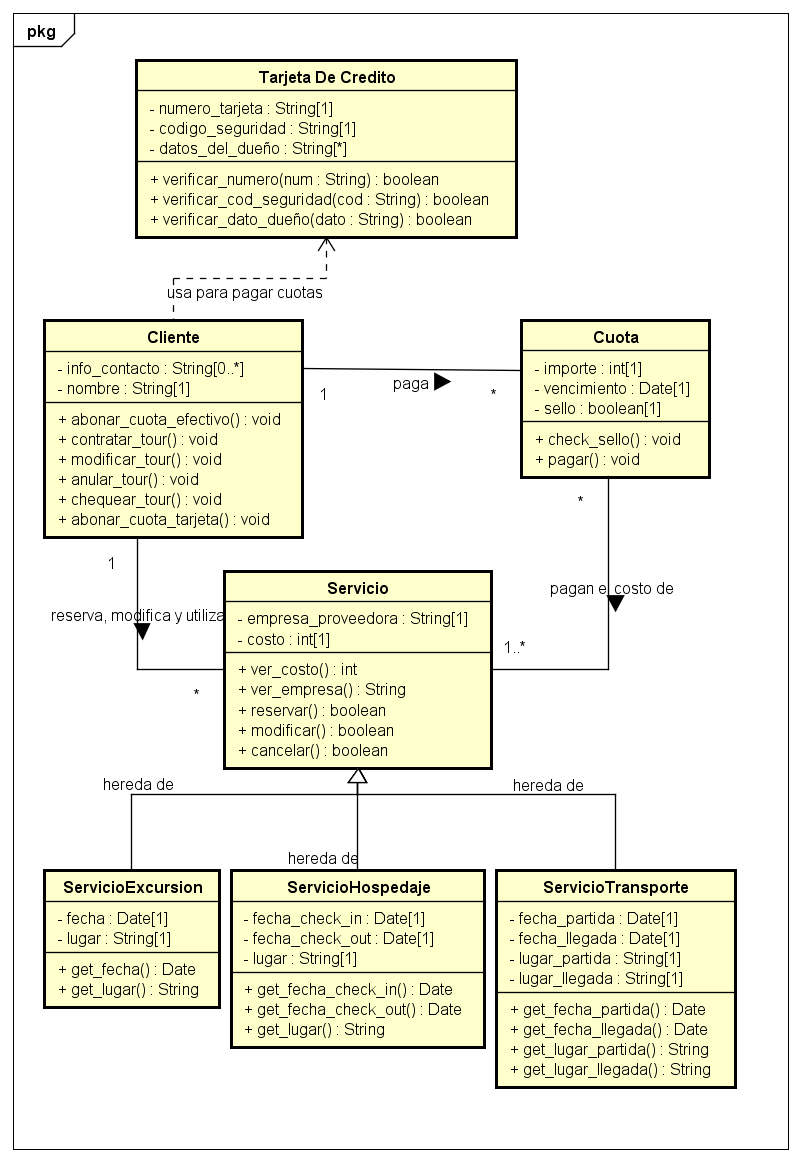
\includegraphics[scale=0.7]{diagramaDeClases.png}

\section{Diagramas de Interacción}
	\subsection{Diagrama de Secuencia}
		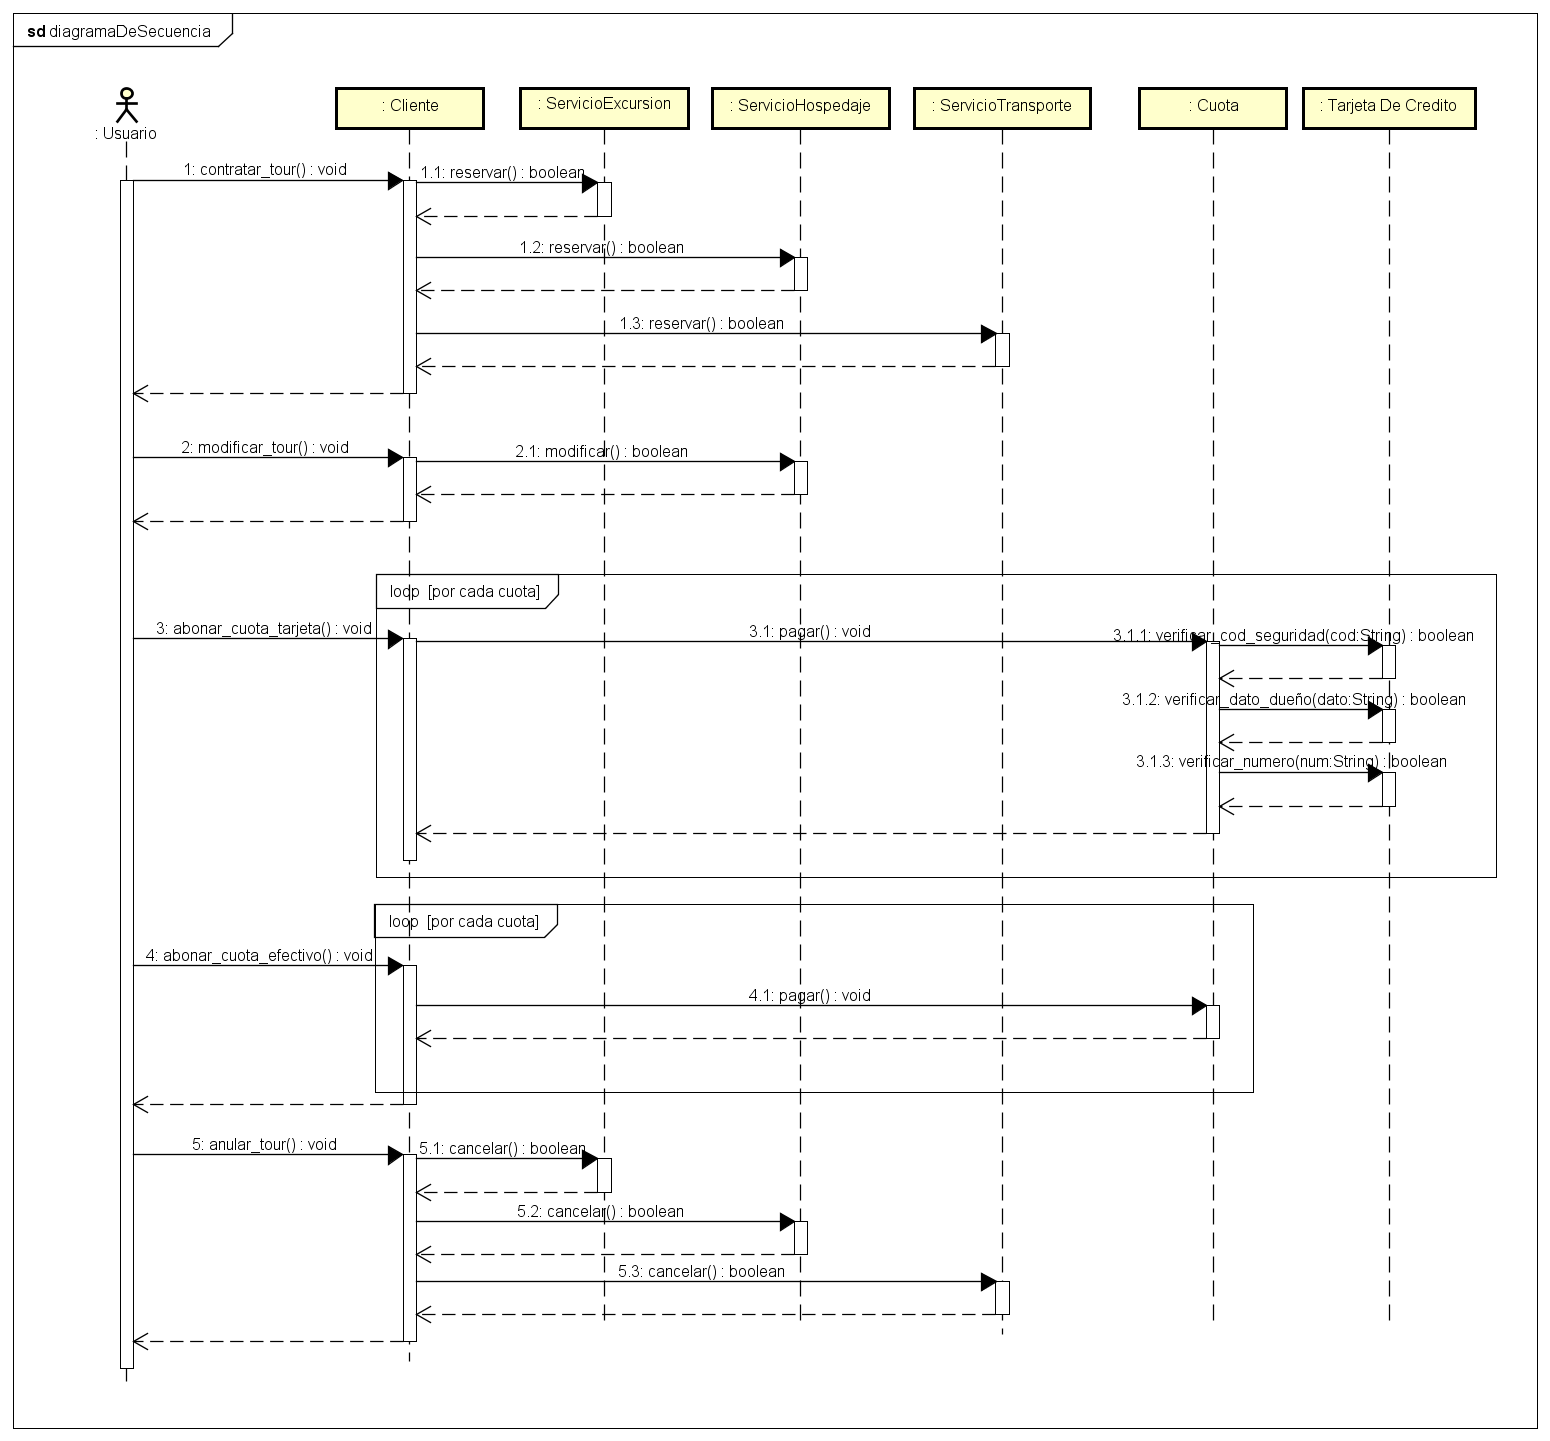
\includegraphics[scale=0.45]{diagramaDeSecuencia.png}

	\subsection{Diagrama de Colaboración}
		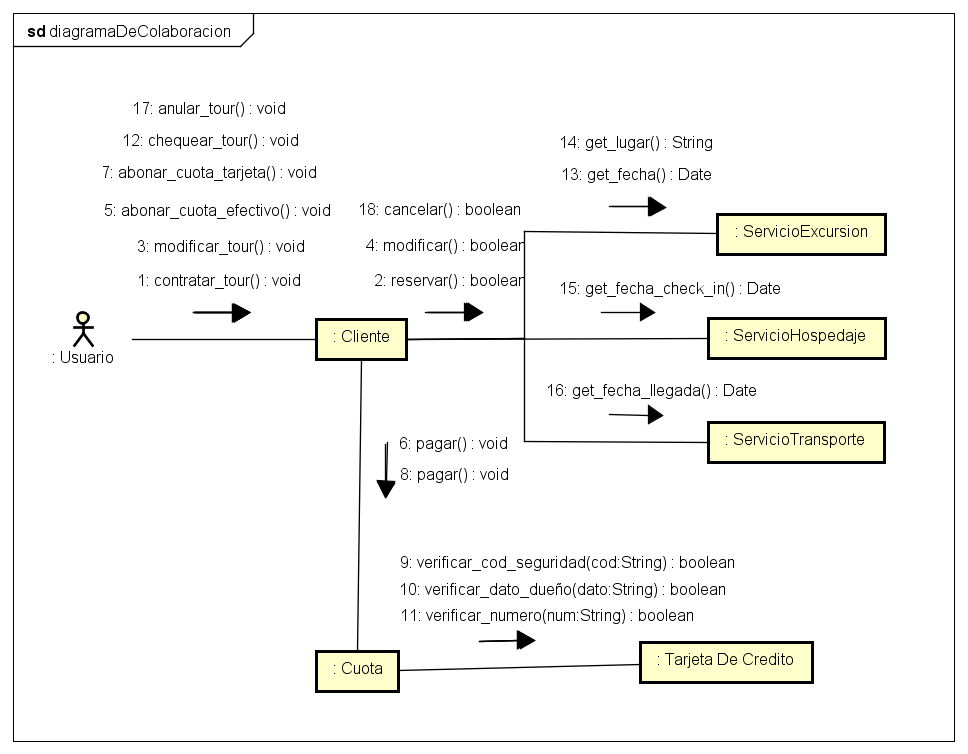
\includegraphics[scale=0.7]{diagramaDeColaboracion.png}
\end{document}